\documentclass[10pt,twocolumn,letterpaper]{article}

\usepackage{statcourse}
\usepackage{times}
\usepackage{epsfig}
\usepackage{graphicx}
\usepackage{amsmath}
\usepackage{amssymb}
\usepackage{enumitem}
\usepackage{pgfplots}
\usepackage{verbatim}
%\newcommand{\source}[1]{\caption*{Source: {#1}} }
\usepackage[hyphens]{url}
\usepackage{paralist}

\setlength{\parskip}{0pt}
\setlength{\parsep}{0pt}
\setlength{\headsep}{0pt}
\setlength{\topskip}{0pt}
\setlength{\topmargin}{0pt}
\setlength{\topsep}{0pt}
\setlength{\partopsep}{0pt}

%\usepackage[margin=0.75in]{geometry}
\everypar{\looseness=-1}
\linepenalty=1000
%\addtolength{\topmargin}{0in}
%\usepackage[compact]{titlesec}
%\linespread{0.97}
%\usepackage[belowskip=-15pt,aboveskip=0pt]{caption}
%\usepackage{titlesec}
%\titlespacing*{\section}{0pt}{1.1\baselineskip}{\baselineskip}
%\usepackage[compact]{titlesec}


% recommended by log
%\pgfplotsset{compat=1.16}

% Include other packages here, before hyperref.

% If you comment hyperref and then uncomment it, you should delete
% egpaper.aux before re-running latex.  (Or just hit 'q' on the first latex
% run, let it finish, and you should be clear).
\usepackage[breaklinks=true,bookmarks=false]{hyperref}


\statcoursefinalcopy


\setcounter{page}{1}
\begin{document}


%%%%%%%%%%%%%%%%%%%%%%%%%%%%%%%%%%%%%%%%%%%%%%%%%%%%%%%%%%%%%%%
% DO NOT EDIT ANYTHING ABOVE THIS LINE
% EXCEPT IF YOU LIKE TO USE ADDITIONAL PACKAGES
%%%%%%%%%%%%%%%%%%%%%%%%%%%%%%%%%%%%%%%%%%%%%%%%%%%%%%%%%%%%%%%



%%%%%%%%% TITLE
\title{MIDTERM REPORT \\ Hate Speech Detection with Deep Learning Models in PyTorch}


\author{Carlos Eduardo Posada\\
{\tt\small c.posada@mpp.hertie-school.org}
\and
Maximilian Kupi\thanks{These authors are sharing the project between the NLP and Python class.}\\
{\tt\small m.kupi@mpp.hertie-school.org}
\and 
Michael Bodnar\\
{\tt\small m.bodnar@mpp.hertie-school.org}
\and
Nikolas Schmidt\footnotemark[1]\\
{\tt\small n.schmidt@mpp.hertie-school.org}}


\maketitle
%\thispagestyle{empty}


% MAIN ARTICLE GOES BELOW
%%%%%%%%%%%%%%%%%%%%%%%%%%%%%%%%%%%%%%%%%%%%%%%%%%%%%%%%%%%%%%%

%%%%%%%%% ABSTRACT
\begin{abstract}
 Hate speech is a growing concern, particularly on social media, and automated methods have so far been sub-par at reliably detecting it. Challenges lie in the evasive nature of hate speech, particularly in the ambiguity and fast evolution of natural language, as well as the lack of consensus on the definition of hate speech. In this paper, we propose a new multi-class classification approach, aiming to address these issues. We implement a Convolutional Neural Network (CNN) architecture, fused with a classification feature based on a dictionary of hateful words in order to classify a dataset of 110,748 tweets into three categories: hateful, abusive, and normal tweets. We utilize the CNN for the classification, by implementing the architecture’s core functionality to detect patterns from word combinations on our dataset, after vectorising the tweets with a pre-trained BERT model. Preliminary results show that the overall performance of the model is well above random chance, but there is still room for improvement. With the dictionary-enriched CNN input, which we will implement after the midterm, we aim to further improve these results and test them against our now newly established baseline.



% An abstract should concisely (200-250 words) motivate the problem, describe your aims, describe your contribution, and highlight your main finding(s). Given that your project is still a work-in-progress, it's OK if `your contribution' and `your findings' are things you're still working on.
\end{abstract}

%%%%%%%%% BODY TEXT

%\begin{comment}
 %   \begin{itemize}
  %  \item Remember that you should \textbf{submit the report}  via Moodle and \textbf{include in the report the link to accessible GitHub repository that contains the code}. Also, \textbf{only one member per team} needs to submit the project material. You must include a link to your GitHub repository for the project as the first footnote on the first page. 
    
   % \item The midterm project report should be {\bf 4 pages long (not counting references), and a maximum 10 references}. The report should contain the sections that are already provided in this paper. It forms the basis of the final report with the same structure. Please check out the text in these sections for further information.
    
    %\item Your midterm milestone will be graded on the following criteria:
    %\begin{itemize}
    %\item Progress: Has the team made good progress on the project? You should have done approximately half of the work of your project.
    %\item As a minimum, your milestone should show that you have setup your data, baseline model code, and evaluation metric, and run experiments to obtain some results (assuming you are doing a typical model-building project). Other than this, `good progress' depends on various factors (e.g., whether your model is implemented from scratch or based on an existing codebase).
    %\item Understanding: Does the milestone show a strong understanding of its problem, tasks, methods, metrics, and research context?
    %\item Writing quality: Does the milestone clearly communicate what you've done and why, providing the requested information, to an appropriate level of detail (given the page limit)?
    %\item You will receive some brief feedback on your milestone. Feedback may contain helpful suggestions for your project (e.g., try a particular method, read a particular paper) and/or warnings about your project plan (e.g., if your plans are too ambitious or not ambitious enough), and how you could improve your technical writing (e.g., adjustments to clarity, level of detail, formatting, use of references).
    %\end{itemize}
    
    %\item Technical writing is an important skill in this class, in research, and beyond. It's well worth spending time developing your ability to communicate technical concepts clearly. Here are some resources which might help you improve your technical writing:
    %\begin{itemize}
    %\item Tips for Writing Technical Papers, Jennifer Widom (\url{https://cs.stanford.edu/people/widom/paper-writing.html}).
    %\item Write the Paper First, Jason Eisner (\url{https://www.cs.jhu.edu/~jason/advice/write-the-paper-first.html}).
    %\end{itemize}
    
    %\item Here are some other things you can do to improve your technical writing:
    %\begin{itemize}
   % \item Look carefully at several ML / NLP papers to understand their typical structure, writing style, and the usual content of the different sections. Model your writing on these examples.
  %  \item Think about the NLP / ML papers you've read (for example, the one you summarised for your proposal). Which parts did you find easy to understand and why? Which parts did you find difficult to understand and why? Can you identify any good writing practices that you could use in your technical writing?
 %   \item Ask a friend to read through your writing and tell you if is clear. This can be useful even if the friend does not have the relevant technical knowledge.
%   \end{itemize}
%    \end{itemize}
%\end{comment}

\section{Proposed Method\protect\footnote{If not further specified, all code for the model as well as for grid search, training and evaluation was written by the authors. The code can be accessed from the following GitHub repository: \url{ https://github.com/MaximilianKupi/nlp-project }.}}

\paragraph{Choice of model:}

Convolutional Neural Network (CNN) architectures typically excel at computer vision and image and video processing, but have also shown promise in Natural Language Processing, and Speech Recognition \cite{Khan2019}.

In Natural Language Processing, other architectures such as Recurrent Neural Networks (RNNs) have also been used, including Gated Recurrent Unit (GRU) and Long Short-Term Memory (LSTM) RNN architectures \cite{Adel2017}.
However, in detecting hate speech, CNNs have been shown to offer distinct advantages over other architectures.%cite Heller paper (not Towards Data Science) here if still space
Namely, CNNs are adept at extracting features and recognising patterns from word combinations, while RNNs rely on features based in sequences. This specificity of CNNs is relevant for hate speech, where certain combinations of words occur often, while the sequence in which certain words occur is less important. Additionally, tweets are short\footnote{140 characters in the data we are using; Twitter changed the maximum character length of a tweet to 280 characters in 2017.}, which makes the capability to detect sequences in a single tweet less useful for our purposes. This is especially relevant, when hate speech is determined by the occurrence of specific words\footnote{This approach in understanding hate speech underpins also our further investigation methods, see Section \ref{Section 3} .}, whereas modeling a longer sequence - such as done with GRU - can miss key words determining the meaning within a sequence \cite{Yin2016}.
Furthermore, CNN architectures have been shown to be more efficient than RNN architectures, as RNNs take longer or more computing power to train \cite{Adel2017}.\footnote{While this may not be an issue in our application, as our data input is limited, striving for efficiency in use of computational power should be a matter of principle.} For these reasons, we've chosen a CNN model architecture to distinguish between hateful, abusive or normal tweets. We implement that architecture in Python, using the PyTorch library \cite{PyTorch2019}.
\paragraph{Convolutional Neural Network:}
CNNs are a special kind of multi-layer perceptron that include additional layers called convolutional layers, in which the process of convolution occurs. In this process, a filter, which is a small matrix of weights, also called a kernel, is applied to the input data in matrix form in order to capture local correlations between points (e. g. spatial and temporal dependencies) \cite{Khan2019}, and at the same time reduce processing complexity and time \cite{Saha2018}. It must be noted that the input matrix and the kernel can be matrices of dimension 1, i.e. vectors. This is of particular relevance for this project, as our input —text— has only one dimension, contrary to images, which have two, for which CNNs were originally developed.

During convolution, the kernel strides over the input matrix. While striding, it is matrix-multiplied with a new section of the input matrix. The results of the multiplication are summed up and after the kernel has stridden over the whole input matrix, a matrix of weighted sums is obtained. This output has reduced complexity over the input dataset and conserves the most essential features, defined by the kernel. The first layers of convolution extract low-level features of the input data, while later layers capture high-level features \cite{Saha2018}.

Padding is another characteristic of the convolution process. It consists of adding extra zero values to the input matrix, so that the kernel can cover its edges equally while striding. When no additional values are added, the process is called valid padding and the convolved matrix will have the same dimensions as the kernel. When extra values are added, the process is called same padding, and the convolved matrix has the same size as the input matrix \cite{Saha2018}.

The hyperparameters that can be set in order to define how the CNN will work are: (1) the size of the kernel, which defines the shape of the convolution; (2) the stride, which controls the size of the steps the kernel will take while displacing over the input matrix; (3) the padding, which defines the size of the convolved matrix; (4) and the dilation, which sets the pattern and distance between each step of matrix multiplication \cite{Rao2019}.

Furthermore, an extra layer, called the pooling layer, can be added after each convolutional layer. The pooling layer further reduces the size of the convolved matrix, producing significant gains in computational efficiency and a reduction in the risk of overfitting \cite{jacovi-etal-2018-understanding}. It “summarises” the convolved matrix by pooling values of the matrix and generating a new matrix with the summary values, usually the maximum values of the pools \cite{Newatia2019}. In the case of text classification, pooling has to be considered carefully, since the redundancy of information in text is lesser than in images.

The final output matrix is flattened into a vector and fed into a multi-layer perceptron, which receives the extracted features and calculates the values for final classification \cite{Newatia2019}. The loss is computed by comparing the predicted and the true labels, in our case, using a multi-class cross-entropy loss function. Finally, the weights of the kernel are adapted based on the loss through backpropagation. This is how the network "learns" \cite{Khan2019}.\par
\paragraph{Convolution - mathematics in 1D:} \label{Subsection 1.3} 
The following explanation is based on the master documentation of PyTorch \cite{PyTorch2019}.

As discussed above, a convolution is used to combine multiple input values with different weights attached to them to an output value. We call the object that contains all the weights used in the calculation a kernel and define it as $w\in\mathbb{R}^n$.

Each layer gets a 1D vector of length $n$ as input. Let the whole input vector be $x\in\mathbb{R}^n$. Based on the settings for kernel size, stride, and dilation the kernel is applied to a sub-sequence $\tilde{x}$ of input vector $x$.

We can define the application of the kernel mathematically as a function that takes the sub-vector $\tilde{x}$ and a vector of weights $w$ to calculate a weighted sum, i.e. the convolution:
$$f:\mathbb{R}^n\times\mathbb{R}^n\rightarrow \mathbb{R}, \hspace{0.3cm}(\tilde{x},w)\mapsto \sum_{i=1}^n w_i x_i =:y_* $$

The initial weights are generated randomly with a uniform distribution of values. All neurons in the first layer get the same input vector but will produce different convolutions due to the randomness of the weights.
If all weights would be equal then the backpropagation algorithm that tweaks the weights after each training step would have to change all of them or choose randomly which one to adjust because all would have the same effect. Randomisation of the weights takes this decision from the algorithm by "breaking symmetry" in the network \cite[p.~297]{Goodfellow-et-al-2016}. Thus, the randomisation is the precondition for the network to learn.

PyTorch calculates the range of values from which it can draw randomly from the amount of input values and the kernel size.
The possible weights must be in the range $(-\sqrt{k},+\sqrt{k})$, where $k:=\frac{1}{\text{input channels}\cdot\text{kernel size}}$.

If we look at all the convolutions happening in order to produce the output of one neuron, we can see that an individual input value is included in multiple weighted sums.
The choice of $k$ ensures that neurons with different kernel size and/or input channel amount produce convolutions that are in the same numerical range. This happens through a kind of normalisation in the definition of $k$.
Each neuron in the neural network has its own weights and draws them randomly from a uniform random distribution, e.g. $w_1,w_2,w_3 \in\mathcal{U}(-\sqrt{k},\sqrt{k})$ like in Figure \ref{fig:initweights}.
\begin{figure}[ht]
    \begin{center}
        \includegraphics[width=5cm,keepaspectratio]{writing/01_midterm-report-latex/figures/intialization.pdf}
        \caption{Random initialisation of kernel weights (own visualisation)}
        \label{fig:initweights}
    \end{center}
\end{figure}



The weights are then used in function $f$ to apply them to the sub-vector. In the following example a sub-vector $\tilde{x}=[x_1,x_2,x_3]$ of length $3$ is convoluted with a weight vector $w=[w_1,w_2,w_3]$ of length $3$. The calculation for one output value of a neutron can be seen in Figure \ref{fig:calculate1}.

\begin{figure}[ht]
    \begin{center}
        \includegraphics[width=5cm,keepaspectratio]{writing/01_midterm-report-latex/figures/1dconvolution.pdf}
        \caption{1D convolution as simple linear equation (own visualisation)}
        \label{fig:calculate1}
    \end{center}
\end{figure}


In each neuron this calculation is repeated for all sub-vectors of the vector (or only a part of it depending on kernel size, stride and dilation). This results in one matrix multiplication per neuron which applies the kernel to each sub-vector and outputs one vector with the result of all the associated convolutions (see Figure \ref{fig:matmult}).

\begin{figure}[ht]
    \begin{center}
        \includegraphics[width=7cm,keepaspectratio]{writing/01_midterm-report-latex/figures/matmult.pdf}
        \caption{Convolution as matrix multiplication (own visualisation)}
        \label{fig:matmult}
    \end{center}
\end{figure}

Finally a bias $b$ is added to the weighted sum. The initial bias $b$ is drawn randomly from the same uniform distribution $\mathcal{U}(-\sqrt{k},\sqrt{k})$.

While the weights $w$ determine the focus of the calculations, the bias $b$ directly influences the result of the activation function of the neuron. If the activation function is a Sigmoid function (see Figure \ref{fig:sigmoid}) then e.g. a simple shift to the left (negative $b$) could reduce the whole neuron output to zero and thus make the information covered in the convolutions irrelevant for the network. The bias puts some neurons' activation threshold lower and some higher in the beginning, and allows the network to focus on the relevant information. As was mentioned above in relation to the weights, the initial randomisation of the bias allows the network to learn.
%
\begin{figure}[ht]
    \begin{center}
        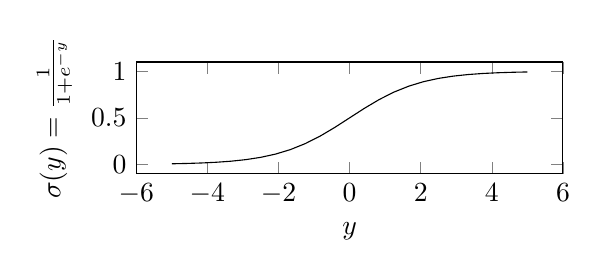
\begin{tikzpicture}
          \begin{axis}[
            height=3cm,
            width=7cm,
            ymax=1.1,
            ymin=-0.1,
            xlabel=$y$,
            ylabel={$\sigma(y) = \frac{1}{1+e^{-y}}$}
          ] 
            \addplot[mark=none] {1/(1+e^(-x))};
          \end{axis}
        \end{tikzpicture}
        \caption{Sigmoid function (own visualisation)}
        \label{fig:sigmoid}
    \end{center}
\end{figure}

%
The weights and the bias are adjusted depending on the loss after each training step through the backpropagation algorithm.

\paragraph{Convolution - from 1D to 2D:} \label{Subsection 1.4} 
The 2D CNN works analogously to the 1D network but inputs and kernels are extended into the second dimension. And thus, a matrix convolution builds weighted sums of numbers spread over the area of a sub-matrices instead of a sequence of numbers of a sub-vector. The second dimension allows to add additional potentially relevant information to each word of the text (see Dictionary approach in Section~\ref{Section 3}).
\paragraph{Data preprocessing:} The tweets were preprocessed in order to remove noise \cite{Lata2018}. The text was transformed to lower case, and punctuation, whitespaces and standalone digits were removed. Tweet-specific traits, such as URLs, mentions, hashtags, reserved words, emojis and smileys were also removed.\footnote{Using the tweet-preprocessor program from Said Özcan: \url{https://pypi.org/project/tweet-preprocessor/}} The tweets were then vectorised using a BERT pretrained model \cite{Devlin2018}. BERT models are bidirectionally trained, so they achieve a better sense of language context than single-directional models. For efficiency and reliability reasons we employ the BERT-base-uncased model \cite{Rajapakse2020}. The maximum vector length has been set to 120 and padded with zeros.\par 
\paragraph{Baseline model architecture:}
As our baseline model we use a CNN architecture with two hidden layers, a ReLU activation function, and batch normalisation after each CNN layer.\footnote{Modelled after a CNN template from:  \url{https://adventuresinmachinelearning.com/convolutional-neural-networks-tutorial-in-pytorch/}} The initial number of channels is set to one, as we input one vector per tweet. The output channels of the first, second, and third CNN layer have been set to 16, 32, and 64, respectively. The out features of the final linear layer have been set to three in order to match the three classes of the tweet annotation. 


\section{Experiments} \label{Section 2} %Max 
\paragraph{Data:}  
%Describe the dataset(s) you are using (provide references). If it's not already clear, make sure the associated task is clearly described.
We use the following two datasets for our classification task:
\begin{compactenum}
\itemsep0em 
    \item The dataset from Davidson et al. \cite{hateoffensive}, which is composed of 25,000 tweets that have been pre-selected using the crowd-sourced "Hatebase" hate speech keyword lexicon (see Section~\ref{Section 3}) and manually labeled using the crowd-sourcing platform CrowdFlower
    \item The dataset from Founta et al. \cite{founta2018large}, which comprises 100,000 manually annotated tweets (again using CrowdFlower) whose annotation has been checked for statistical robustness by the authors 
\end{compactenum}

The datasets have the following labelling categories:
\begin{compactitem}
\itemsep0em 
    \item Davidson et al.: hate\_speech, offensive\_language, neither
    \item Founta et al.: hateful, abusive, normal, spam
\end{compactitem}

Since our focus does not lie on spam detection, we decided to delete all tweets in this category from the second dataset. Next, following the definitions of Founta et al. \cite{founta2018large}, according to which offensive and abusive language are two very similar categories, we decided to merge both datasets. The benefits of doing so are a more balanced dataset\footnote{Both original datasets had a significant class imbalance between all three classes, while the resulting dataset is more balanced – at least between the classes normal, and abusive (see Figure~\ref{fig:counts}).} as well as an increased sample size for the hate class, which was highly underrepresented in both datasets. Since the resulting dataset, composed of 110,748 tweets, was still rather unbalanced with respect to the 'hate' category (see Figure~\ref{fig:counts}), we used a stratified shuffle split, to finally divide our dataset into training (70\%), validation (15\%), and test set (15\%), while ensuring that the classes would be distributed equally amongst all splits. 
\begin{figure}[ht]
    \begin{center}
        \includegraphics[width=8cm,keepaspectratio]{writing/01_midterm-report-latex/figures/dataset_merging.pdf}
        \caption{Counts for the respective classes in the datasets}
        \label{fig:counts}
    \end{center}
\end{figure}

\paragraph{Evaluation method:} As a first metric to evaluate the results of our model, we observed the evolution of the accuracy on the training and validation set over the training epochs. This gave a first hint on whether the model was training correctly. Furthermore, the decrease of the training and validation loss over the epochs was used as an indication for the model's convergence and generalisability. However, since accuracy tends to be highly misleading due to the class imbalance of the dataset, we further paid particular attention to the F1 macro score and also took into account the F1 score for the least represented 'hate' class.

\paragraph{Experimental details:} To determine the best hyperparameters for our model, we made use of a grid search. We specified the following variables for the grid search:
\begin{compactitem}
\itemsep0em 
    \item optimizer type (Adam, RMSprop, and SGD)
    \item learning rate (0.0001, 0.001, 0.01)
    \item whether to use a sampler in the data loader or class weights in the loss function to balance the dataset during training\footnote{In case the class weights were used, the shuffle mode in the data loader was automatically set to true in order to ensure more robust training.}
    \item whether or not to use a scheduler to decrease the learning rate (factor 0.1) based on the performance of the F1 macro score
\end{compactitem}
During grid search we trained each model for 30 epochs with a batch size of 16. We then considered the results from the best epoch with respect to the F1 macro score. Based on the results from the grid search the best overall model was selected and retrained for 90 epochs. This yielded the loss plot shown in Figure~\ref{fig:loss}. As can be seen, the model saturates after around 45 epochs and the validation loss is lower than the training loss, which could be due to different calculations of the batch normalisation during training and validation.
%
\begin{figure}[h!]
    \begin{center}
        \includegraphics[width=8cm,keepaspectratio]{writing/01_midterm-report-latex/figures/loss_90epochs.pdf}
        \caption{Loss plot of best model over 90 epochs}
        \label{fig:loss}
    \end{center}
\end{figure}
%
%%%%% Test Michael
%\includegraphics[width=8cm,keepaspectratio]{writing/01_midterm-report-latex/figures/test.pdf}
%%%%% End Test Michael
\paragraph{Results:} 
The best model from the grid search turned out to have the following specifications: Adam optimizer, 0.01 learning rate, class weights in the loss function, and activated scheduler. After retraining this model for 90 epochs, the highest F1 macro score was yielded in epoch 37. Table~\ref{tab: classification report} shows the respective classification report. 
%
\begin{table}[ht]
\begin{center}
\begin{tabular}{r c c c c}
& \textit{Precision} & \textit{Recall} & \textit{F1 Score} \\

 hate & 0.21 & 0.26 & 0.23\\
abusive   &    0.69   &   0.67   &   0.68 \\
normal    &   0.75    &  0.75   &   0.75 \\
 \textit{Accuracy}      & & & 0.69 \\
\textit{ Macro Avg }    &  0.55    &  0.56     & 0.55 \\
 \textit{Micro Avg}   &    0.69   &   0.69  & 0.69 

\end{tabular}
\end{center}
\caption{Classification report of the best model (epoch 37 of 90)}
\label{tab: classification report}
\end{table}
%
As can be seen in the classification report as well as in the confusion matrix (see Figure~\ref{fig:confusion matrix}), the overall performance of the model is way above random chance. Yet, in comparison to Davidson et al. \cite{hateoffensive}, who trained classifiers on the smaller subset of our data and yielded an overall precision, recall and F1 score of above 0.90 with their best models, our performance metrics seem rather low.\footnote{Since they framed their problem as a one-versus-rest problem, these score are best compared to the micro F1 score.} However, since Davidson et al. did not apply a deep neural network architecture for classification – instead they used linear support vector machines and logistic regression – and framed the problem as a one-versus-rest classification, which eradicated the problem of class imbalance completely, these results are hardly comparable. 
%
\begin{figure}[h!]
    \begin{center}
        \includegraphics[width=8cm,keepaspectratio]{writing/01_midterm-report-latex/figures/confusion_matrix.pdf}
        \caption{Confusion matrix of the best model (epoch 37 of 90)}
        \label{fig:confusion matrix}
    \end{center}
\end{figure}
%
\section{Future work} \label{Section 3} % Michael, Niko
% Michael: Math of 2d CNN + Dictionary and explaining Visualisation 
% Niko: Dictionary non-math part - basically done


% Describe what you plan to do for the rest of the project, and why. You can include stretch goals if you like.

In order to further improve our model's performance, in particular with respect to correctly distinguishing hate speech from normal tweets (see confusion matrix in Figure~\ref{fig:confusion matrix}), we are planning to implement the following additional feature into our model architecture:
\paragraph{Adding information retrieved from the "Hatebase" dictionary to the second input dimension:}
The project "Hatebase"\footnote{\url{https://www.hatebase.org}} includes manually collected, tagged and described hate speech terms in multiple languages, which are used in incidents of hate speech in real public online conversations. For the purposes of our model, we have extracted the English-language entries, compiling a dictionary of hateful terms. During the preprocessing, we will check each word in each tweet in our dataset against this dictionary and generate a two-fold output: 
\begin{compactitem}
\itemsep0em 
    \item A vector containing a 0/1-classification (1: hate term, 0: not a hate term) for each word
    \item A vector of numerical values indicating the level of hatefulness of each word calculated based on Hatebase's classifications of each term's average offensiveness as well as the unambiguity as a hateful term.
\end{compactitem}



These vectors will then be transformed into tensors and attached to the tensor which was created with BERT from the original tweets. The resulting matrix will then be used as an input for the 2D-architecture for our model.

This additional, innovative element should improve our model performance, since it offers the possibility of more clearly classifying tweets in which unambiguously hateful terms are used.

So far, dictionaries / lexicons of hateful terms have mostly been utilized in rule-based machine classification \cite{Martins2018}. For example, in order to select potentially (!) hateful content (such as tweets) from a database of content to establish a baseline or to assess the quality of classification of crowd-sourced manual tagging \cite{hateoffensive}.\footnote{Note that, while part of our data was already selected using Hatebase, this applies to only 20\% of our data. Furthermore, we are using the current version of Hatebase, which will result in better detection, since Hatebase is continuously updated.} Furthermore, to our knowledge, none of these approaches has taken into account an ambiguity measure as provided by the Hatebase dictionary.

Depending on the results of this approach and overall project progress, we might also use the first output in a different way – namely to not only use a 0/1-classification for each word, but to also count the number of hate terms in each tweet, as it has been suggested that most hateful content contains multiple hateful slurs \cite{hateoffensive}.
For our future work the model results presented in this report will serve as a baseline.
\newpage
{\small
\bibliographystyle{IEEEtran}
\bibliography{writing/references.bib}
}

\end{document}
